%----------------------------------------------------------------------------
\appendix
%----------------------------------------------------------------------------
\chapter*{Függelék}
\setcounter{chapter}{6}  % a fofejezet-szamlalo az angol ABC 6. betuje (F) lesz
\setcounter{equation}{0} % a fofejezet-szamlalo az angol ABC 6. betuje (F) lesz
\numberwithin{equation}{section}
\numberwithin{figure}{section}
\numberwithin{lstlisting}{section}
\numberwithin{table}{section}
\setcounter{footnote}{0}

%,,,,,,,,,,,,,,,,,,,,,,,,,,,,,,,,,,,,,,,,,,,,,,,,,,,,,,,,,,,,,,,,,,,,,,,,,,,,
\section{Paraméterezés}\label{sect:parameterezes}
%,,,,,,,,,,,,,,,,,,,,,,,,,,,,,,,,,,,,,,,,,,,,,,,,,,,,,,,,,,,,,,,,,,,,,,,,,,,,

blabla fv hogy van parameterzve

\newpage
%,,,,,,,,,,,,,,,,,,,,,,,,,,,,,,,,,,,,,,,,,,,,,,,,,,,,,,,,,,,,,,,,,,,,,,,,,,,,
\section{Bővített osztálydiagram}\label{sect:osztalydiagram}
%,,,,,,,,,,,,,,,,,,,,,,,,,,,,,,,,,,,,,,,,,,,,,,,,,,,,,,,,,,,,,,,,,,,,,,,,,,,,

\begin{figure}[!ht]
\centering
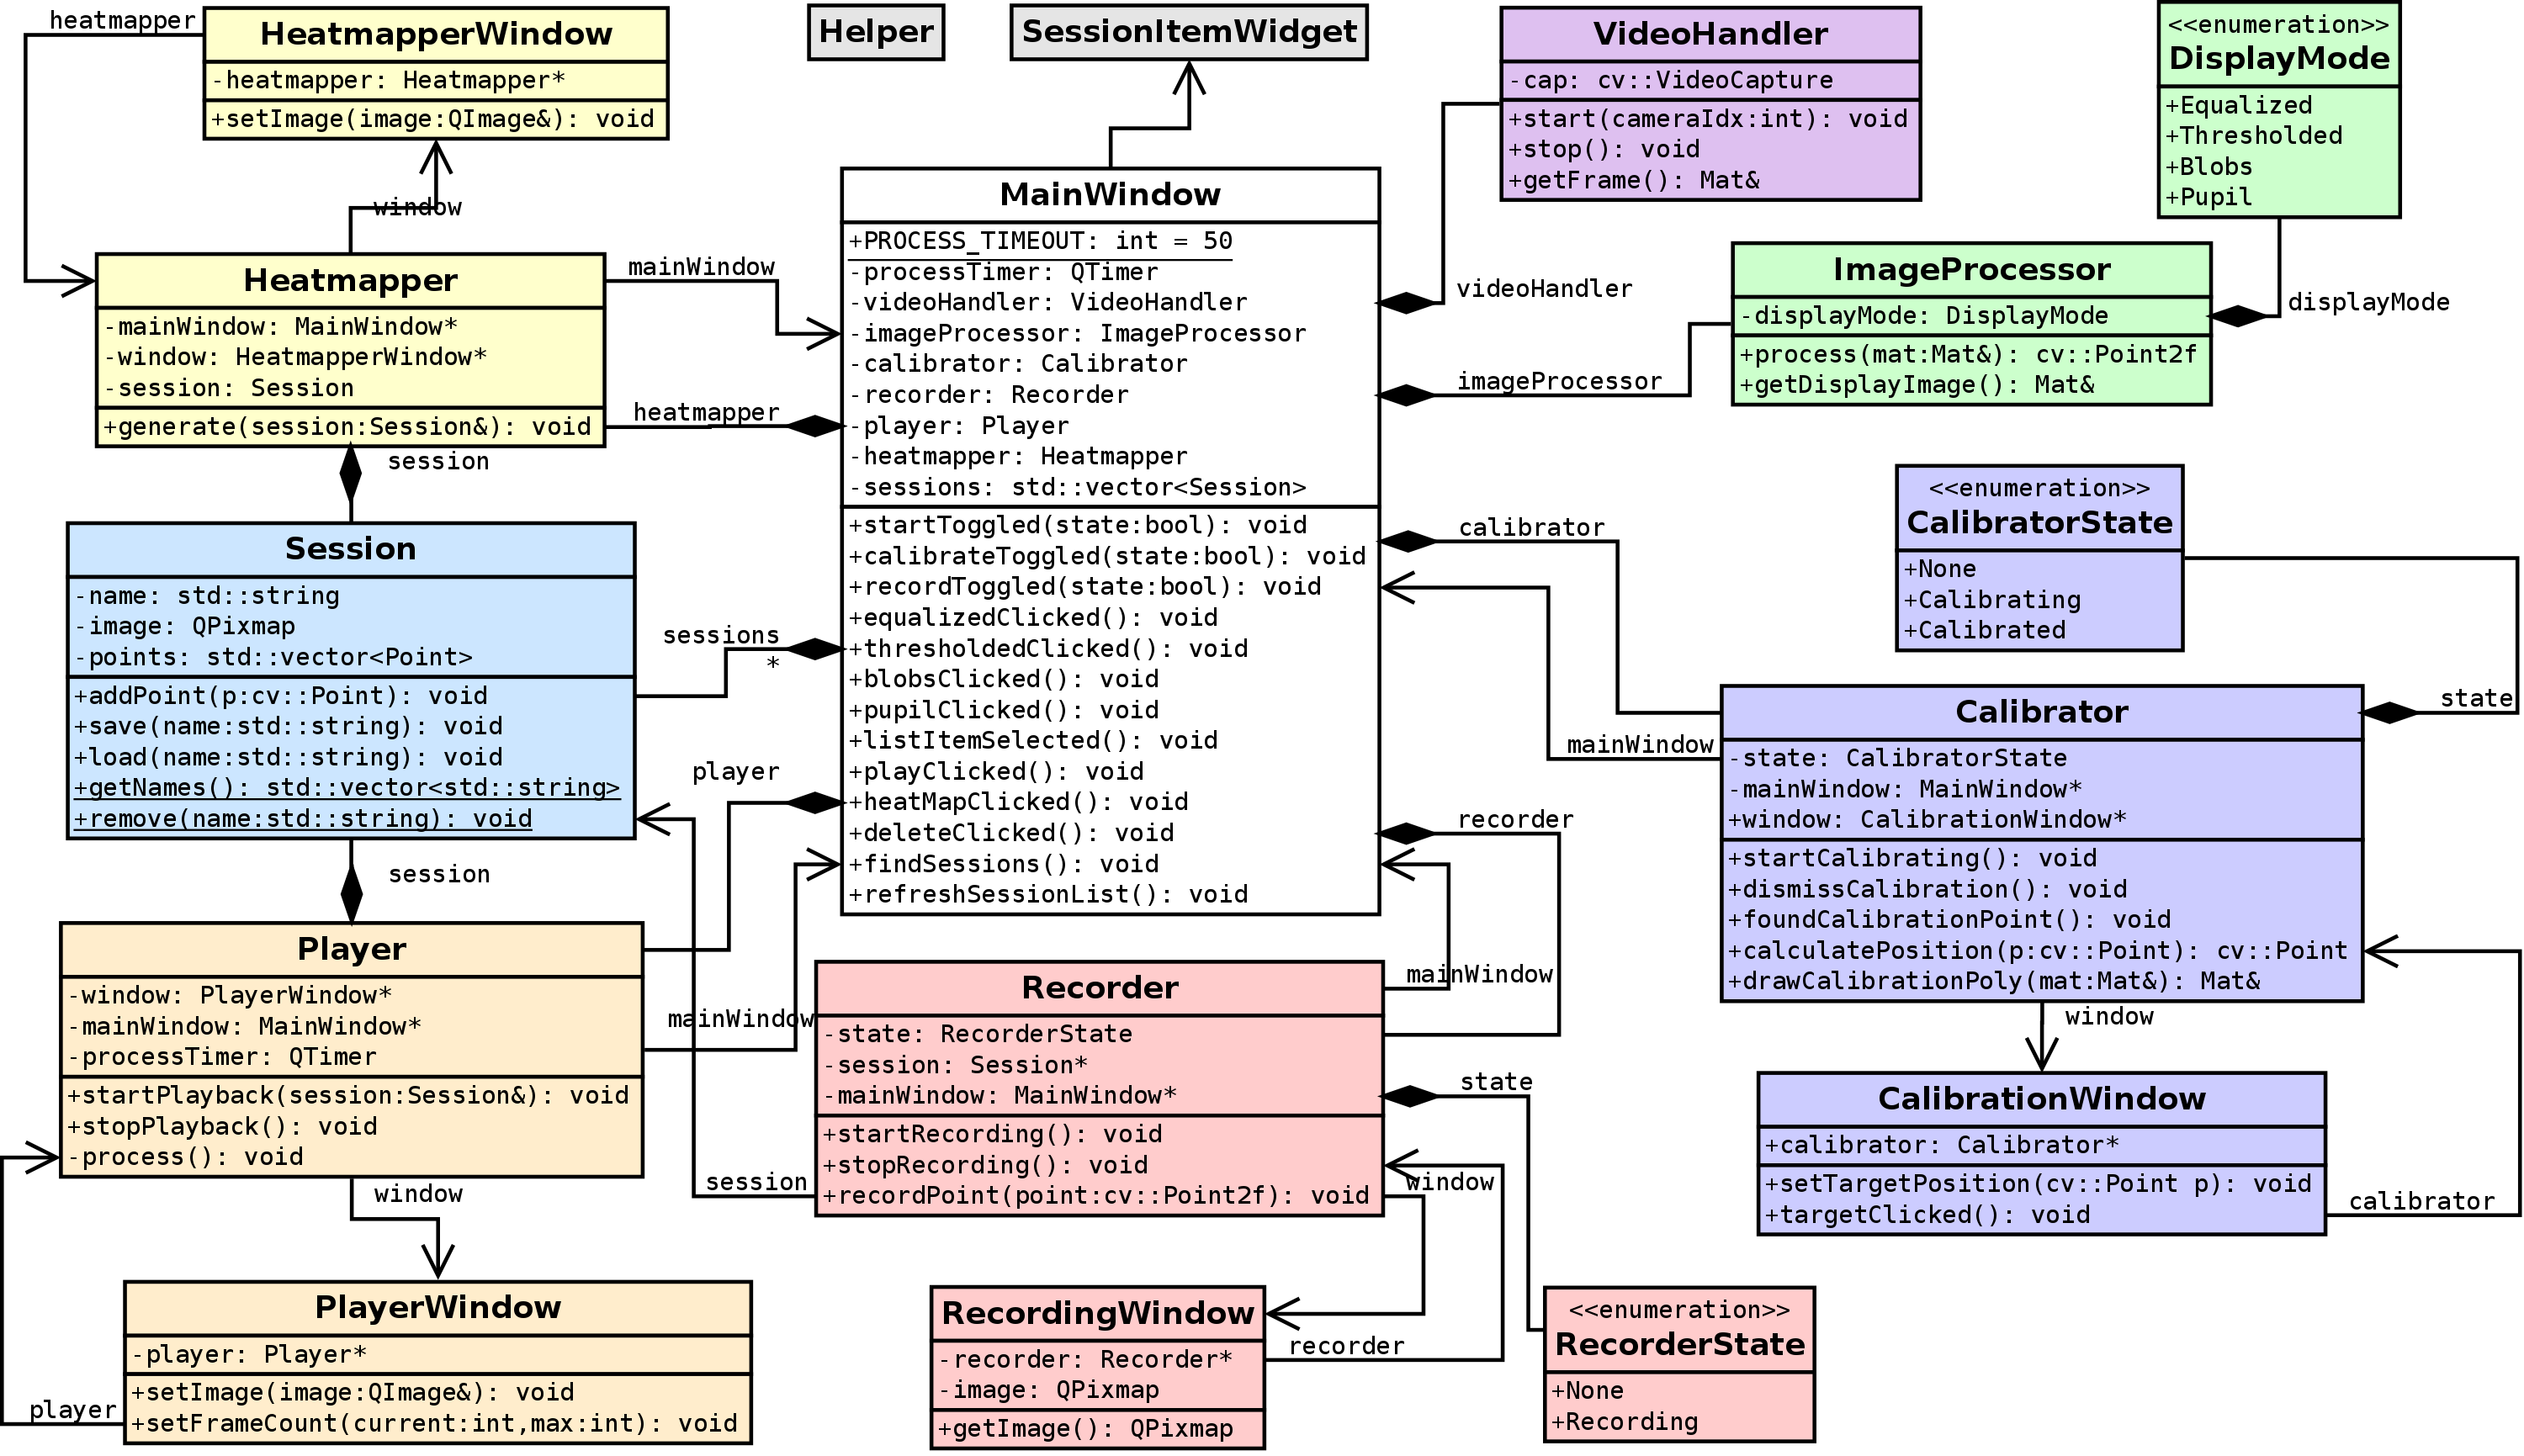
\includegraphics[width=130mm, keepaspectratio]{figures/class_diagram_aa.png}
\end{figure}


\newpage
%,,,,,,,,,,,,,,,,,,,,,,,,,,,,,,,,,,,,,,,,,,,,,,,,,,,,,,,,,,,,,,,,,,,,,,,,,,,,
\section{Telepítés}\label{sect:telepites}
%,,,,,,,,,,,,,,,,,,,,,,,,,,,,,,,,,,,,,,,,,,,,,,,,,,,,,,,,,,,,,,,,,,,,,,,,,,,,

\texttt{+++ forditas menete, szukseges szoftverek +++}

%Az alkalmazás fordítása az alábbi verziójú programokkal történt:

%\begin{itemize}
%\item g++ --  4.4.5
%\item OpenCV -- 2.1.0
%\item wxWidgets -- 2.8.10
%\end{itemize}

%A  2.1.0 verziójú \textit{OpenCV} könyvtár forráskódja az \url{http://opencv.willowgarage.com/wiki/} címről letölthető. Az ennél újabb verziók interfészébe nem került bele a működéshez elengedhetetlenül szükséges \texttt{cvSnakeImage} függvény, ezért az alkalmazás mindenképpen a fenti verziójú \textit{OpenCV} könyvtár meglétét igényli! A fordításhoz szükséges csomagok a használt disztribúció csomagkezelőjéből elérhetők az \listref{install} listában felsorolt (vagy ahhoz hasonló) néven.

%\begin{lstlisting}[frame=single,float=!ht,caption=Az OpenCV fordításához szükséges csomagok telepítése,label=listing:install]
%sudo apt-get install libgtk2.0-dev libunicap2-dev libucil2-dev libswscale-dev \\
%libdc1394-22-dev libv4l-dev libxine-dev libavformat-dev libglut3-dev \\
%libwxgtk2.8-dev
%\end{lstlisting}

%A \emph{Pupil Measure} alkalmazás fordítása ezek után a forráskód könyvtárában kiadott \texttt{make} paranccsal történhet. A lefordított bináris a \texttt{./pupilmeasure} parancs kiadásával indítható, de előtte az \texttt{LD\_LIBRARY\_PATH} környezeti változóba a \texttt{usr/local/lib} érték betöltendő!
